\documentclass{altsu-report}
\linespread{1,15}
\title{Генератор персонажа DnD}
\author{А.\,В.~Лаптев}
\groupnumber{595}
\GradebookNumber{1337}
\supervisor{И.\,А.~Шмаков}
\supervisordegree{ст. преп.}
\ministry{Министерство науки и высшего образования}
\country{Российской Федерации}
\fulluniversityname{ФГБОУ ВО Алтайский государственный университет}
\institute{Институт цифровых технологий, электроники и физики}
\department{Кафедра вычислительной техники и электроники}
\departmentchief{В.\,В.~Пашнев}
\departmentchiefdegree{к.ф.-м.н., доцент}
\shortdepartment{ВТиЭ}
\abstractRU{Цель работы --- разработка программного продукта под микроконтроллер одного из рассмотренных семейств AVR или ARM, на выбранной программной и аппаратной платформах.

В результате выполнения научно-исследовательской работы было создано приложение для генерации персонажа Dangeous \& Dragons с использованием аппаратно-программной платформы Arduino.}
\abstractEN{Большой текст на английском!}
\keysRU{AVR, ARM, Arduino, микроконтроллер, генератор персонажа DnD}
\keysEN{computer simulation, distributed version control}

\date{\the\year}

% Подключение файлов с библиотекой.
\addbibresource{graduate-students.bib}

\begin{document}
\begin{titlepage}
 \begin{center}
    \normalsize
    МИНИСТЕРСТВО НАУКИ И ВЫСШЕГО ОБРАЗОВАНИЯ \\
    РОССИЙСКОЙ ФЕДЕРАЦИИ \\
    ФГБОУ ВО «АЛТАЙСКИЙ ГОСУДАРСТВЕННЫЙ УНИВЕРСИТЕТ»
    \vfill
     
    Институт цифровых технологий, электроники и физики (ИЦТЭФ) \\
    Кафедра вычислительной техники и электроники (ВТиЭ)
    \vfill
     
    \textbf{Генератор персонажа Dangeons \& Dragons на платформе Arduino} \\
    Отчет по научно-исследовательской работе
 \end{center}
\vfill
 
\newlength{\ML}
\settowidth{\ML}{«\underline{\hspace{3cm}}»}
\hfill\begin{minipage}{0.41\textwidth}
  Выполнил: студент 595 гр.\\
  \underline{\hspace{\ML}} А.\,В.~Лаптев \\
  Проверил: ст. преп. кафедры ВТиЭ\\
  \underline{\hspace{\ML}} И.\,А.~Шмаков \\
  «\underline{\hspace{1cm}}» \underline{\hspace{3cm}} 2022 г.
\end{minipage}%
\vfill
 
\begin{center}
  Барнаул, 2022 г.
\end{center}
\end{titlepage}

\setcounter{page}{2}
\makeabstract
\tableofcontents

\chapter*{Введение}
\addcontentsline{toc}{chapter}{Введение}

На сегодняшний день практически у каждого есть какое-либо портативное устройство или другая потребительская электроника. В такой технике приоритетом является низкое энергопотребление в сочетании с относительным быстродействием. Этим требованиям отвечают семейства микроконтроллеров AVR и ARM.

Сейчас встраиваемые системы и портативные устройства --- одна из самых быстрорастущих технологических сфер. И, поэтому, разработка под микроконтроллеры и микропроцессоры этих семейств является актуальной.

Целью данной работы является разработка программного продукта под микроконтроллер одного из рассмотренных семейств, с использованием выбранной программной и аппаратной платформ.

Задачи работы:

\begin{enumerate}
    \item Рассмотрение имеющихся аппаратных и программных средств для выбора наиболее подходящей платформы для разработки под AVR и ARM микроконтроллеры.
    
    \item Разработка собственного программного продукта на выбранной аппаратно-программной платформе.
\end{enumerate}

\chapter{Краткий обзор платформ}

Для облегчения разработки под микроконтроллеры имеет смысл использовать готовые отладочные платы, поскольку на них есть не только микроконтроллер, но и набор обвязки, необходимый для его нормальной работы.

На сегодняшний день существует довольно много аппаратных и программных платформ для разработки под микроконтроллеры.

Среди представителей в аппаратной части можно выделить следующих:

\begin{enumerate}
    \item LaunchPad --- аппаратная платформа, включающая в себя платы с микроконтроллером и платы расширения, производства Texas Instruments. Платформа позиционируется как конкурент Arduino. Специально под LaunchPad была разработана программная платформа Enrgia~\cite{LaunchPad, TI}.
    
    \item STM Nucleo --- семейство отладочных плат от STMicroelectronics на основе микроконтроллеров STM32. Функциональность плат может быть расширена путем подключения плат расширения для Arduino, поскольку она совместима со многими ее компонентами~\cite{Nucleo, STM}.
    
    \item Mbed --- аппаратная часть имеет в своем составе отладочные платы от ARM и других компаний:  семейства плат mbed и FRDM от NXP Semiconductors, семейство Nucleo от STMicroelectronics, семейство EFM32 от Silicon Labs и другие~\cite{Mbed}.
    
    \item Arduino --- аппаратная часть представляет собой набор плат с микроконтроллером и платы расширения. Большинство плат с микроконтроллером снабжено минимально необходимым набором обвязки для нормальной работы микроконтроллера. Сторонними производителями выпускаются различные датчики и устройства, совместимые с Arduino~\cite{wikiRUArduino}.
\end{enumerate}

Среди представителей в программной части существуют следующие варианты:

\begin{enumerate}
    \item Atmel Studio --- интегрированная платформа разработки, предназначенная для проектирования и отладки приложений для микроконтроллеров Atmel на базе микроконтроллеров AVR и ARM. В Atmel Studio поддерживаются следующие языки программирования: C/C++, ассемблер~\cite{MK_2}. IDE имеет все необходимое для комфортного и быстрого написания кода, а также, является гибко настраиваемой. Данное решение является абсолютно бесплатным~\cite{Atmel}.
    
    \item MPLAB --- интегрированная среда разработки для контроллеров производства Microchip. Данная среда поддерживает разработку программ, написанных на C и ассемблере. Имеет множество дополнительных функций и модулей, которые упрощают процесс разработки, отладки и тестирования программ и папку с шаблонами программ на ассемблере, с которыми удобно начинать работу. Распространяется бесплатно~\cite{MPLAB}.
    
    \item Mbed (онлайн IDE) --- в программной части, платформа включает в себя интегрированную среду разработки, которая работает онлайн. Среда включает в себя компилятор, набор библиотек, текстовый редактор и примеры программного кода. Поддерживается облачное хранение кода системой контроля версий Mercurial~\cite{Mbed}.
    
    \item Arduino IDE --- программная часть платформы, которая представляет собой бесплатную IDE, в которую помимо инструментов для разработки включены также инструменты для загрузки программы в микроконтроллер. В основе среды лежит фреймворк Wiring, оболочка написана на основе проекта Processing на Java~\cite{wikiRUArduino}.
    
    \item Energia --- программная платформа для прототипирования электроники с открытым исходным кодом, создана для интеграции с аппаратной платформой LaunchPad от Texas Instruments. Как и Arduino IDE, использует в своей основе фреймворк Wiring и оболочку, написанную на основе проекта Processing, поэтому их интерфейсы схожи~\cite{Energia, ENERGIA}.
\end{enumerate}

Среди всех этих представителей выделяется платформа Arduino, которая, в свою очередь, включает в себя как программную платформу для разработки под микроконтроллеры (среда разработки Arduino IDE), так и аппаратную (большой выбор отладочных плат с различными микроконтроллерами в своем составе,а также плат расширения к ним).

Помимо этого, для программирования в данной платформе используется модифицированный язык C, который называют Arduino C, который довольно хорошо описан на сегодняшний день и проще в освоении, чем чистый C.

Также, платформа имеет довольно большое сообщество разработчиков и производителей аппаратной части, благодаря которому существует множество сторонних библиотек и Arduino-совместимых плат от других производителей, что делает разработку на этой платформе более доступной и комфортной.

Благодаря этому, данная платформа больше подходит для людей, которые не имеют достаточного опыта разработки под микроконтроллеры, в связи с чем эта платформа и была выбрана для реализации данного программного продукта.

\chapter{Генератор персонажа Dangeons \& Dragons (DnD)}
\section{Правила генерации}

Генерация персонажа представляет собой совокупность из параметров персонажа, которые пользователь может выбрать из предложенных вариантов, а также характеристик, которые одинаковы для всех персонажей, но значения которых генерируются случайным образом.

Изначально, пользователю предоставляется возможность выбрать то, кем он, непосредственно, хочет быть в игре (раса и класс персонажа)~\cite{D&D}. После чего происходит генерация значений для характеристик персонажа.

Для определения значений характеристик персонажа существует несколько различных способов~\cite{DnD, DnDWiki}. В данном случае, характеристики персонажа генерируются следующим образом:
\begin{enumerate}
    \item для каждой из характеристик производится четыре броска игральной кости;
    
    \item меньшее из выброшенных значений исключается из генерации;
    
    \item оставшиеся три значения суммируются. Полученное значение и будет являться значением для характеристики.
\end{enumerate}

Для некоторых других характеристик персонажа, таких как хит\-поинты и класс защиты, генерация осуществляется иначе.

Для расчета хит-поинтов для героя первого уровня берется максимальное значение кости хитов, которое определяется классом выбранного персонажа и модификатор телосложения, который рассчитывается исходя из соответствующей характеристики. Полученные значения складываются, что и дает количество хит-поинтов персонажа.

Для расчета класса защиты для героя первого уровня используется значение 10 (базовое значение для персонажа, который не носит броню) и модификатор ловкости, рассчитанный исходя из характеристики ловкости. Данные значения складываются, выводя значение, которое и определяет класс защиты персонажа.

Модификаторы телосложения, ловкости и других характеристик рассчитываются одинаково. Формула для расчета модификатора конкретной характеристики выглядит следующим образом: $MC = (CH - 10) / 2$, где MC --- модификатор характеристики, CH --- конкретное значение характеристики, для которого производится расчет. Полученный результат округляется в меньшую сторону. Модификатор характеристики может принимать значение от $-5$ до $+10$~\cite{D&D_forms}.

\section{Реализация генератора персонажа DnD}

Генератор персонажа реализован на отладочной плате Arduino Uno, в основе которой лежит микроконтроллер ATmega328. Для отображения меню генерации персонажа и навигации по нему используется плата расширения LCD Keypad Shield (Arduino-совместимая), на которой располагается LCD-дисплей 16x2, а также набор кнопок, которые могут быть использованы, непосредственно, для навигации. Разработка генератора персонажа велась с использованием интегрированной среды разработки Arduino IDE.

В генераторе реализованы следующие возможности:

\begin{enumerate}
    \item возможность выбора расы персонажа.
    
    \item Возможность выбора класса персонажа.
    
    \item Генерация случайных значений для характеристик персонажа, согласно правилам DnD.
    
    Базовые характеристики персонажа DnD:
    
    \begin{itemize}
        \item Сила (Strong --- сокращенно <<Str>>);
        
        \item Телосложение (Constitution --- сокращенно <<Con>>);
        
        \item Ловкость (Dexterity --- сокращенно <<Dex>>);
        
        \item Интеллект (Intelligence --- сокращенно <<Int>>);
        
        \item Мудрость (Wisdom --- сокращенно <<Wis>>);
        
        \item Харизма (Charisma --- сокращенно <<Cha>>).
    \end{itemize}
    
    \item Расчет количества Хит-поинтов (Hit Points --- сокращенно <<HP>>) персонажа на основе сгенерированных характеристик.
    
    \item Расчет Класса Защиты (Armor Class --- сокращенно <<AC>>) персонажа с использованием сгенерированных характеристик.
\end{enumerate}

Для реализации данного набора возможностей решение было разбито на функции, каждая из которых отвечает за выбор параметров персонажа или за генерацию значений его характеристик.

\subsection{Функция mainText}

Эта функция представляет собой реализацию приветственного окна, в котором сообщается о назначении программы (генератор персонажа DnD) и указывается, что для продолжения работы нужно нажать соответствующую кнопку.

Помимо этого, после нажатия кнопки внутри функции генерируются псевдослучайные числа, которые имитируют броски игральной кости. Генерируется четыре псевдослучайных числа и находится сумма этих чисел, исключая меньшее. Такие манипуляции производятся шесть раз (по количеству характеристик персонажа). Блок-схема подпрограммы mainText изображена на рис.~\ref{fig:main1},~\ref{fig:main2} в Приложении А.

\subsection{Функция genRacePers}

В этой функции реализована часть генератора, которая отвечает за выбор пользователем расы персонажа. На экран выводятся двенадцать вариантов рас, среди которых пользователь может переключаться нажатием на кнопки: <<ВВЕРХ>> (<<UP>>), <<ВНИЗ>> (<<DOWN>>), <<ВПРАВО>> (<<RIGHT>>), <<ВЛЕВО>> (<<LEFT>>); чтобы подтвердить свой выбор требуется нажать кнопку <<ВЫБРАТЬ>> (<<SELECT>>). Блок-схема подпрограммы genRacePers (см. рис.~\ref{fig:race1},~\ref{fig:race2} в Приложении А).

\subsection{Функция genClassPers}

В этой функции реализована возможность выбора класса персонажа. На экран последовательно выводятся тринадцать предусмотренных классов, между которыми также можно переключаться с помощью кнопок, для подтверждения выбора предусмотрена кнопка <<ВЫБРАТЬ>> (<<SELECT>>). Блок-схема подпрограммы genClassPers изображена на рис.~\ref{fig:class1},~\ref{fig:class2} в Приложении А.

\subsection{Функция charactPers}

С помощью данной функции на экран выводятся значения характеристик, сгенерированные в функции mainText, а также на их основе высчитываются количество хит-поинтов и класс защиты для выбранных расы и класса, которые также выводятся на экран. Навигация здесь, также как и в предыдущих функциях осуществляется с помощью кнопок. Блок-схема подпрограммы charactPers изображена на рис.~\ref{fig:char1},~\ref{fig:char2} в Приложении А.

\subsection{Функция clickButton}

Эта функция необходима для того, чтобы обрабатывать нажатия кнопок, она возвращает целое число, которое будет указывать на то, нажата ли кнопка и, если нажата, то какая. Блок-схема подпрограммы clickButton изображена на рис.~\ref{fig:click} в Приложении А.

Помимо этих функций в проектах, написанных в Arduino IDE есть еще две стандартных функции. В функции setup задается скорость передачи данных для последовательного порта и инициализируется lcd-дисплей. В функции loop вызывается функция mainText для того, чтобы генератор персонажа работал вплоть до отключения его от питания. Блок-схемы алгоритмов подпрограмм loop и setup изображены на рис.~\ref{fig:setup},~\ref{fig:loop} в Приложении А.

\subsection{Недостатки разработанного генератора персонажа DnD}

Полученный скетч использует 6395~байт памяти устройства, что составляет примерно 19~\% от общего объема памяти. Глобальные переменные, в свою очередь, используют 678 байт динамической памяти, что составляет примерно 33~\% от ее объема. Такие показатели не являются оптимальными для подобной программы и на то есть несколько причин.

Во-первых встроенные функции в Arduino IDE зачастую имеют в своем составе ряд дополнительных проверок, чтобы минимизировать количество возможных ошибок, которые могут появиться при компиляции, что, в свою очередь, расходует довольно значительную часть ресурсов~\cite{hate}.

Во-вторых, довольно большое количество глобальных переменных, а также их не оптимальная типизация, из-за которой они могут занимать в памяти больше места, чем им требуется в действительности, также увеличивают количество потребляемых ресурсов микроконтроллера и, как следствие, уменьшают общее быстродействие и производительность.

Также на работу программы негативное влияние оказывает использование встроенной функции задержки delay, поскольку, при использовании этой функции, приостанавливается работа всей программы~\cite{millis}. Для задержек больше подходят прерывания либо другая функция --- millis, которая указывает сколько времени нужно <<обходить>> тот блок кода, выполнение которого необходимо приостановить.

\chapter*{Заключение}
\addcontentsline{toc}{chapter}{Заключение}

В ходе выполнения научно-исследовательской работы было проведено знакомство с различными платформами для разработки под микроконтроллеры, проведен обзор различных семейств микроконтроллеров и выбрана платформа для разработки собственного программного продукта --- генератора персонажа DnD.

Были решены основные поставленные задачи, среди которых:

\begin{enumerate}
    \item наличие возможности выбора расы персонажа;
    
    \item наличие возможности выбора класса персонажа;
    
    \item генерация случайных значений для характеристик персонажа, согласно правилам DnD;
    
    \item расчет некоторых дополнительных характеристик персонажа с использованием значений, сгенерированных для основных характеристик.
\end{enumerate}

В результате чего, был разработан вариант генератора персонажа DnD.

Поскольку в данном генераторе реализованы лишь базовые возможности, то в будущем есть возможность для добавления в генератор ряда функций, например, выбор снаряжения на основе выбранного класса или расчет бросков атаки и урона персонажа, чтобы сделать генератор пригодным для полноценного создания персонажа и облегчения расчетов во время игры.

Кроме того, отладочная плата имеет довольно большие габариты и часть периферии не используется, в будущем планируется развести и вытравить собственную плату для уменьшения габаритов устройства, также возможна замена дисплея на больший по размерам, поскольку количество строк и символов в строке дисплея на плате расширения не позволяет пользователю комфортно работать с ним.

\newpage
\addcontentsline{toc}{chapter}{Список использованной литературы}
\printbibliography[title={Список использованной литературы}]

\chapter*{Приложение}
\addcontentsline{toc}{chapter}{Приложение}

%\begin{minted}[fontsize=\footnotesize]{c++}
\begin{code}
\captionof{listing}{Исходный код приложения}
\label{code:pi-example}
\begin{minted}[mathescape,linenos,frame=lines,breaklines]{C++}
#include <LiquidCrystal.h>

LiquidCrystal lcd(8, 9, 4, 5, 6, 7); // Пины для подключения lcd-дисплея

#define BTN_R 1
#define BTN_U 2
#define BTN_D 3
#define BTN_L 4
#define BTN_S 5
#define BTN_NONE 10

int i = 0;
int j = 0;
int k = 0;
int sel;
int characteristics[] = {0, 0, 0, 0, 0, 0, 0, 0};
char* characteristicsPers[] = {"Race: ", "Class: ", "Str: ", "Con: ", "Dex: ", "Int: ", "Wis: ", "Cha: ", "HP: ", "AC: "};
char* racePers[] = {"Human", "Dwarf", "Elf", "Half-orc", "Gnome", "Goliath", "Halfling", "Genasi", "Tiefling", "Aasimar", "Eladrin", "Dragonborn"};
char* classPers[] = {"Bard", "Barbarian", "Fighter", "Wizard", "Druid", "Cleric", "Artificer", "Warlock", "Monk", "Paladin", "Rogue", "Ranger", "Sorcerer"};
char* pers[] = {"", ""};

//Стрелка вврех
byte arrowUp[8] = {
  0b00000,
  0b00000,
  0b00100,
  0b01110,
  0b11111,
  0b00000,
  0b00000,
  0b00000
};

//Стрелка вниз
byte arrowDown[8] = {
  0b00000,
  0b00000,
  0b00000,
  0b11111,
  0b01110,
  0b00100,
  0b00000,
  0b00000
};

//Обработка нажатой клавици
int clickButton() {
  int keyAnalog = analogRead(A0);
  
  if (keyAnalog < 100) {
    // Значение меньше 100 – нажата кнопка right
    return BTN_R;
  } else if (keyAnalog < 200) {
    // Значение больше 100 (иначе мы бы вошли в предыдущий блок результата сравнения, но меньше 200 – нажата кнопка UP
    return BTN_U;
  } else if (keyAnalog < 400) {
    // Значение больше 200, но меньше 400 – нажата кнопка DOWN
    return BTN_D;
  } else if (keyAnalog < 600) {
    // Значение больше 400, но меньше 600 – нажата кнопка LEFT
    return BTN_L;
  } else if (keyAnalog < 800) {
    // Значение больше 600, но меньше 800 – нажата кнопка SELECT
    return BTN_S;
  } else {
    // Все остальные значения (до 1023) будут означать, что нажатий не было
    return BTN_NONE;
  }
}

//Текст в главном окне
void mainText() {
  int roll;
  int randRoll = 0;
  int characteristic;
  
  lcd.setCursor(0, 1);
  lcd.print("Press the 'SELECT' button");
  lcd.home();
  lcd.print("Character generator DnD");
  delay(500);

  int btnSel = 0;
  for (int j = 0; j < 9; j++) {
    btnSel = clickButton();
    if (btnSel == 5) {
      break;
    }
    lcd.scrollDisplayLeft();
    delay(500);
  }

  switch (btnSel){  //Действия при нажатии кнопки SELECT
    case BTN_S:
      randomSeed(millis()); // Генерируем псевдослучайное число (каждый раз различное)
      for (int i = 0; i < 6; i++) { //Определяем значение для характеристики
        roll = 6;
        characteristic = 0;
        for (int j = 0; j < 4; j++) { //Для определения одной характеристики надо провести 6 бросков
          randRoll = random(1, 7);  //Симулируем бросок игральной кости
          if (randRoll < roll) {  //Осуществляем поиск минимального значения среди выброшенных
            roll = randRoll;
            characteristic += randRoll;
          }
          else
          {
            characteristic += randRoll;
          }
        }
        characteristics[i] = characteristic - roll; //Отбрасываем наименьшее значение
      }
      delay(500);
      lcd.clear();
      while(true) {
        lcd.home();
        genRacePers();  //Вызов функции для выбора расы
      }
      break;
    default:
      break;
  }
  lcd.clear();
}

//Выбор расы персонажа
void genRacePers() {
  if(i == 0) {
    lcd.print("Select race:");
    lcd.setCursor(0, 1);
    lcd.print(racePers[i]);
    lcd.createChar(2, arrowDown);
    lcd.setCursor(15, 1);
    lcd.print(char(2));
  }
  else if(i == 11) {
    lcd.print("Select race:");
    lcd.setCursor(0, 1);
    lcd.print(racePers[i]);
    lcd.createChar(1, arrowUp);
    lcd.setCursor(15, 0);
    lcd.print(char(1));
  }
  else {
    lcd.print("Select race:");
    lcd.setCursor(0, 1);
    lcd.print(racePers[i]);
    lcd.createChar(1, arrowUp);
    lcd.setCursor(15, 0);
    lcd.print(char(1));
    lcd.createChar(2, arrowDown);
    lcd.setCursor(15, 1);
    lcd.print(char(2));
  }
  delay(150);

  int btnRacePers = clickButton();
  switch (btnRacePers){
    case BTN_R:
      lcd.clear();
      i++;
      if (i > 11)
        i--;
      break;
    case BTN_U:
      lcd.clear();
      i--;
      if (i < 0)
        i++;
      break;
    case BTN_D:
      lcd.clear();
      i++;
      if (i > 11)
        i--;
      break;
    case BTN_L:
      lcd.clear();
      i--;
      if (i < 0)
        i++;
      break;
    case BTN_S:
      pers[0] = racePers[i];  //Запоминаем выбранную расу
      lcd.clear();
      while(true) {
        lcd.home();
        genClassPers(); //Вызываем функцию выбора класса
      }
      break;
    default:
      break;
  }
  lcd.clear();
}

//Функция выбора класса персонажа
void genClassPers() {
  if(j == 0) {
    lcd.print("Select class:");
    lcd.setCursor(0, 1);
    lcd.print(classPers[j]);
    lcd.createChar(2, arrowDown);
    lcd.setCursor(15, 1);
    lcd.print(char(2));
  }
  else if(j == 12) {
    lcd.print("Select class:");
    lcd.setCursor(0, 1);
    lcd.print(classPers[j]);
    lcd.createChar(1, arrowUp);
    lcd.setCursor(15, 0);
    lcd.print(char(1));
  }
  else {
    lcd.print("Select class:");
    lcd.setCursor(0, 1);
    lcd.print(classPers[j]);
    lcd.createChar(1, arrowUp);
    lcd.setCursor(15, 0);
    lcd.print(char(1));
    lcd.createChar(2, arrowDown);
    lcd.setCursor(15, 1);
    lcd.print(char(2));
  }
  delay(150);

  int btnClassPers = clickButton();
  switch (btnClassPers){
    case BTN_R:
      lcd.clear();
      j++;
      if (j > 12)
        j--;
      break;
    case BTN_U:
      lcd.clear();
      j--;
      if (j < 0)
        j++;
      break;
    case BTN_D:
      lcd.clear();
      j++;
      if (j > 12)
        j--;
      break;
    case BTN_L:
      lcd.clear();
      j--;
      if (j < 0)
        j++;
      break;
    case BTN_S:
      pers[1] = classPers[j]; //Запоминаем выбранный класс
      lcd.clear();
      while(true) {
        lcd.home();
        charactPers();  //Вызываем функцию для просмотра сгенерированных характеристик
      }
      break;
    default:
      break;
  }
  lcd.clear();
}

//Функция для просмотра сгенерированных характеристик
void charactPers() {
  int HP;
  int AC;

  //Определяем количество хит-поинтов персонажа
  if ((pers[1] == classPers[0]) || (pers[1] == classPers[4]) || (pers[1] == classPers[5]) || (pers[1] == classPers[6]) || (pers[1] == classPers[7]) || (pers[1] == classPers[8]) || (pers[1] == classPers[10])) {
    HP = 8 + floor((characteristics[1] - 10) / 2);
  }
  else if (pers[1] == classPers[1]) {
    HP = 12 + floor((characteristics[1] - 10) / 2);
  }
  else if ((pers[1] == classPers[2]) || (pers[1] == classPers[9]) || (pers[1] == classPers[11])) {
    HP = 10 + floor((characteristics[1] - 10) / 2);
  }
  else {
    HP = 6 + floor((characteristics[1] - 10) / 2);
  }
  characteristics[6] = HP;

  //Определяем класс защиты персонажа
  AC = 10 + floor((characteristics[2] - 10) / 2);
  characteristics[7] = AC;
  
  if(k == 0) {
    lcd.print("Characteristics:");
    lcd.setCursor(0, 1);
    lcd.print(characteristicsPers[k]);
    lcd.print(pers[k]);
    lcd.createChar(2, arrowDown);
    lcd.setCursor(15, 1);
    lcd.print(char(2));
  }
  else if(k == 1) {
    lcd.print("Characteristics:");
    lcd.setCursor(0, 1);
    lcd.print(characteristicsPers[k]);
    lcd.print(pers[k]);
    lcd.createChar(1, arrowUp);
    lcd.setCursor(15, 0);
    lcd.print(char(1));
    lcd.createChar(2, arrowDown);
    lcd.setCursor(15, 1);
    lcd.print(char(2));
  }
  else if(k == 9) {
    lcd.print("Characteristics:");
    lcd.setCursor(0, 1);
    lcd.print(characteristicsPers[k]);
    lcd.print(characteristics[k - 2]);
    lcd.createChar(1, arrowUp);
    lcd.setCursor(15, 0);
    lcd.print(char(1));
  }
  else {
    lcd.print("Characteristics:");
    lcd.setCursor(0, 1);
    lcd.print(characteristicsPers[k]);
    lcd.print(characteristics[k - 2]);
    lcd.createChar(1, arrowUp);
    lcd.setCursor(15, 0);
    lcd.print(char(1));
    lcd.createChar(2, arrowDown);
    lcd.setCursor(15, 1);
    lcd.print(char(2));
  }
  delay(150);

  int btnCharPers = clickButton();
  switch (btnCharPers){
    case BTN_R:
      lcd.clear();
      k++;
      if (k > 9)
        k--;
      break;
    case BTN_U:
      lcd.clear();
      k--;
      if (k < 0)
        k++;
      break;
    case BTN_D:
      lcd.clear();
      k++;
      if (k > 9)
        k--;
      break;
    case BTN_L:
      lcd.clear();
      k--;
      if (k < 0)
        k++;
      break;
    default:
      break;
  }
  lcd.clear();
}

void setup() {
  lcd.begin(16, 2); // Инициализация текстового дисплея 16х2
}

void loop() {
  mainText(); //Вызов функции для отображения текста на главном экране
}
\end{minted}
\end{code}

\textbf{Блок-схемы подпрограмм}

\begin{figure}[H]
    \centering
    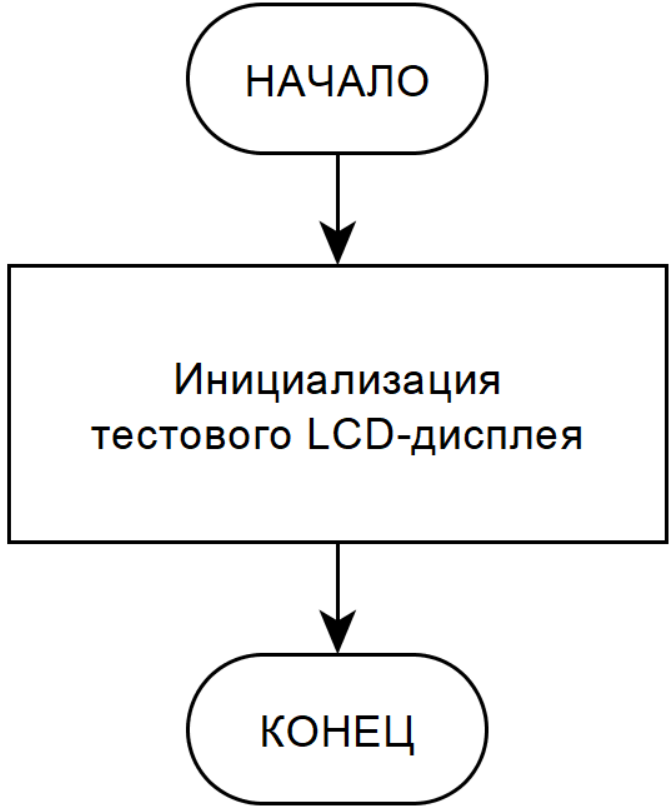
\includegraphics[scale=0.3]{setup.png}
    \caption{Блок-схема функции setup}
    \label{fig:setup}
\end{figure}

\begin{figure}[H]
    \centering
    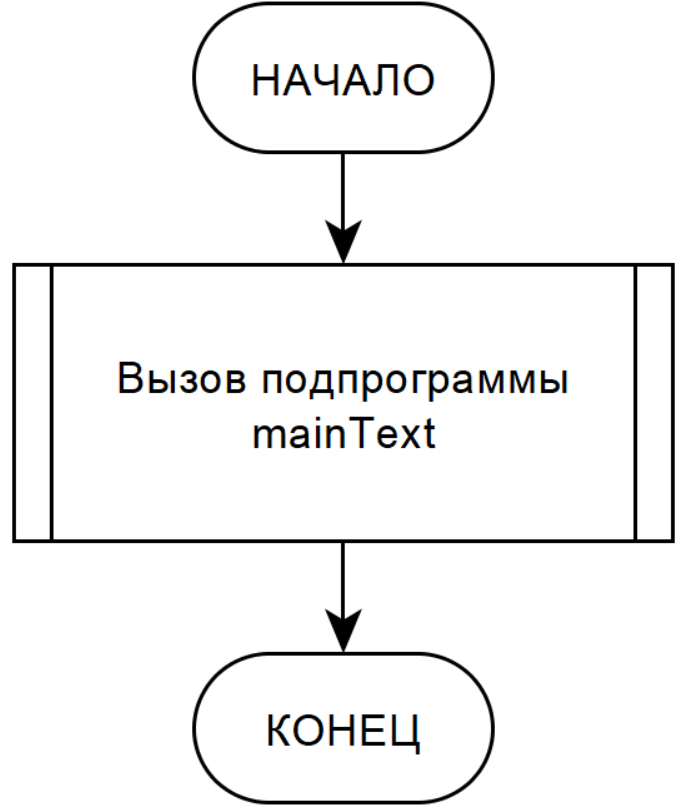
\includegraphics[scale=0.3]{loop.png}
    \caption{Блок-схема функции loop}
    \label{fig:loop}
\end{figure}

\begin{figure}[H]
    \centering
    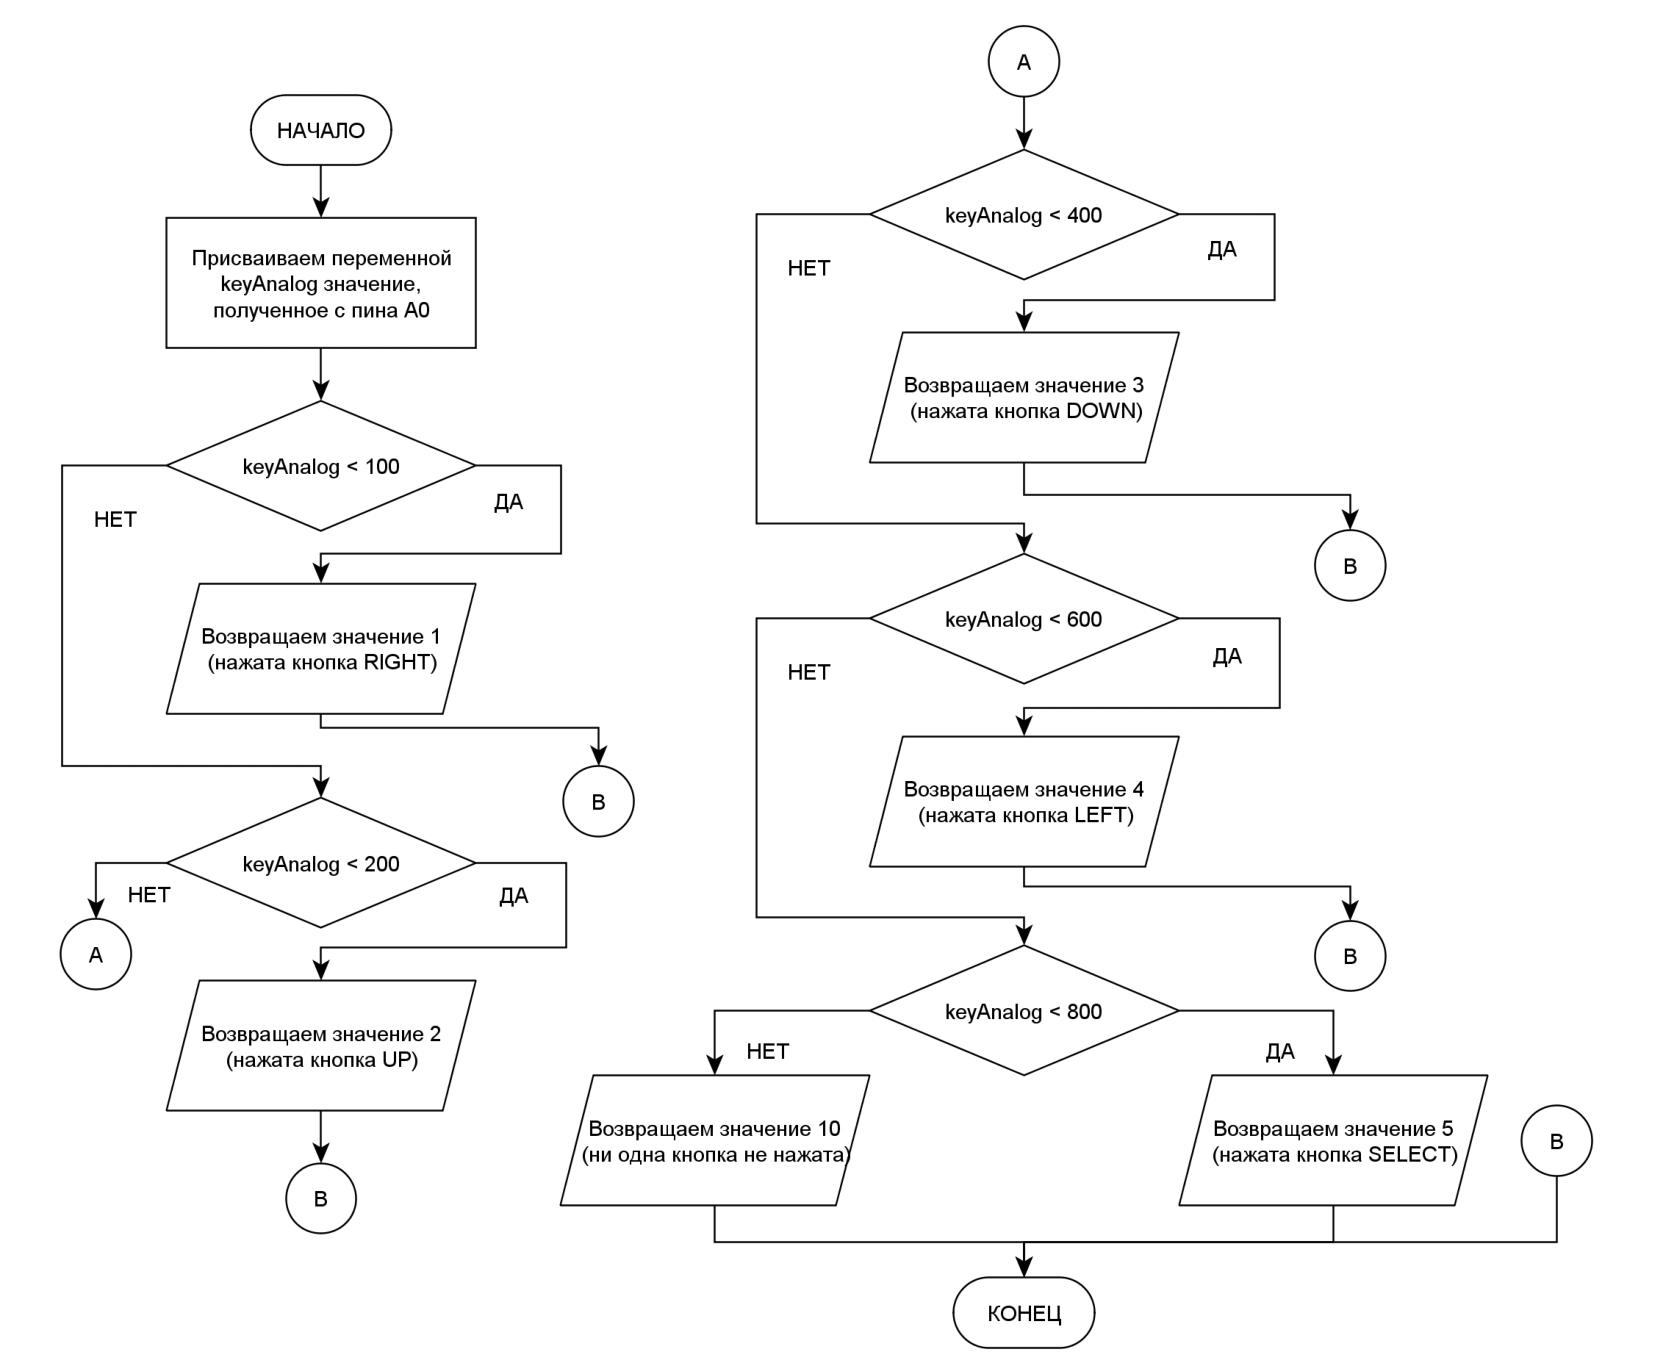
\includegraphics[scale=0.8]{clickButton.png}
    \caption{Блок-схема функции clickButton}
    \label{fig:click}
\end{figure}

\begin{figure}[H]
    \centering
    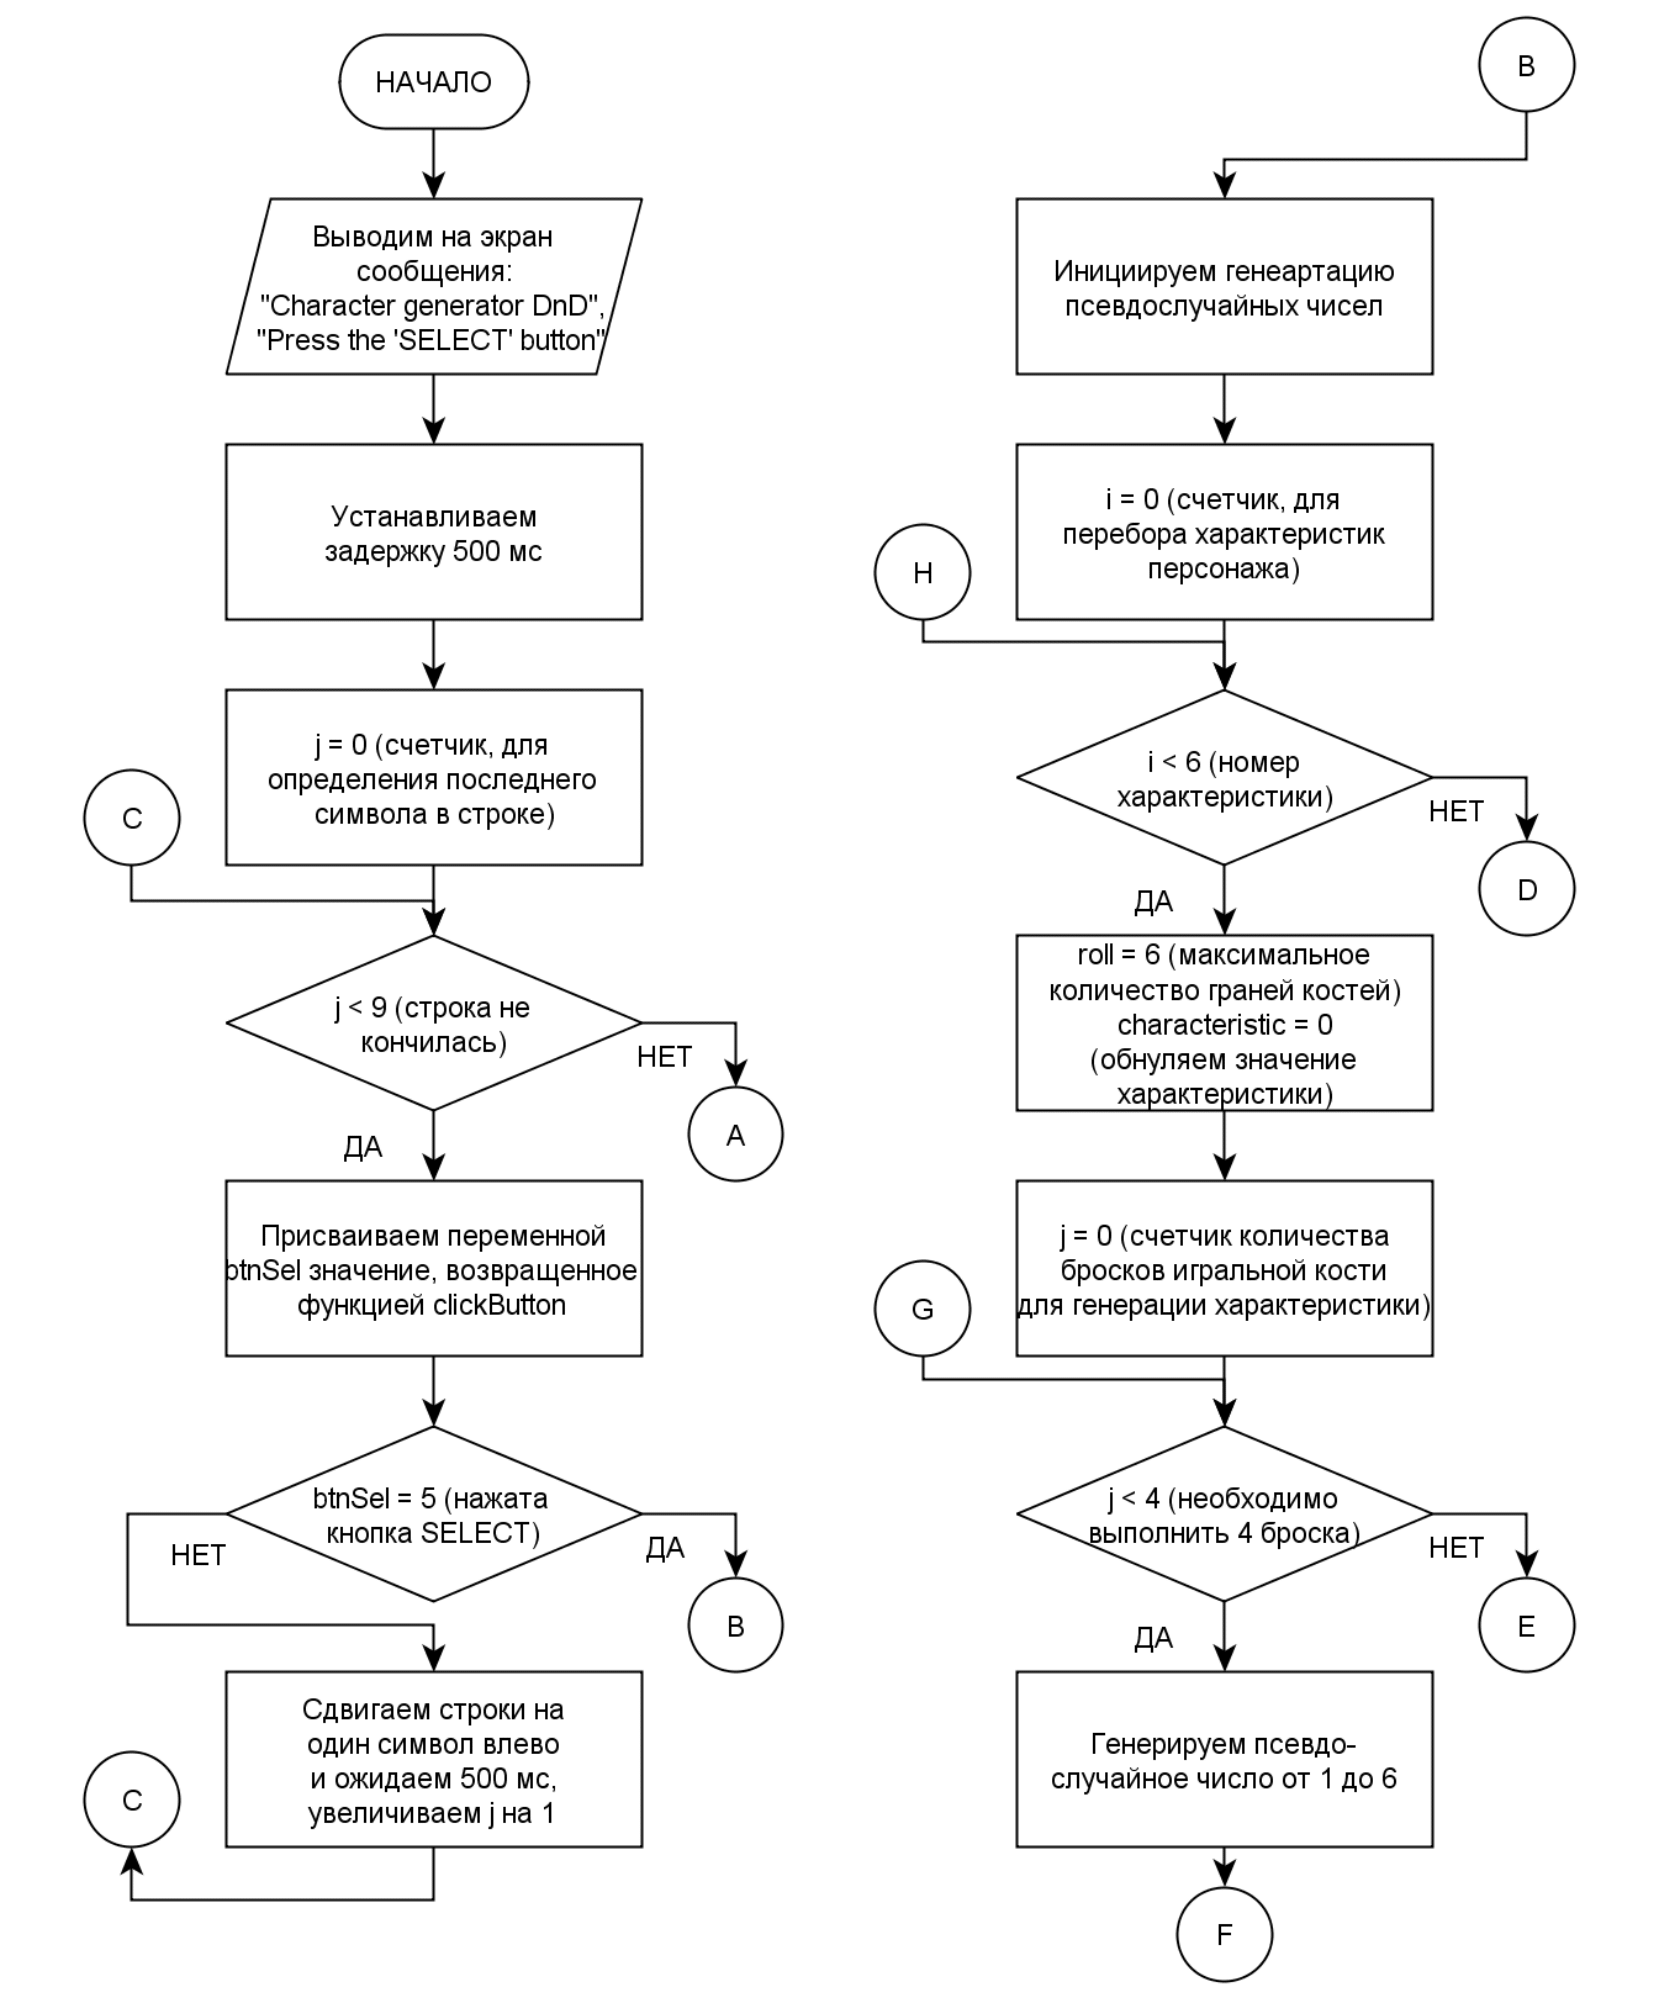
\includegraphics[scale=0.8]{mainText1.png}
    \caption{Блок-схема функции mainText}
    \label{fig:main1}
\end{figure}

\begin{figure}[H]
    \centering
    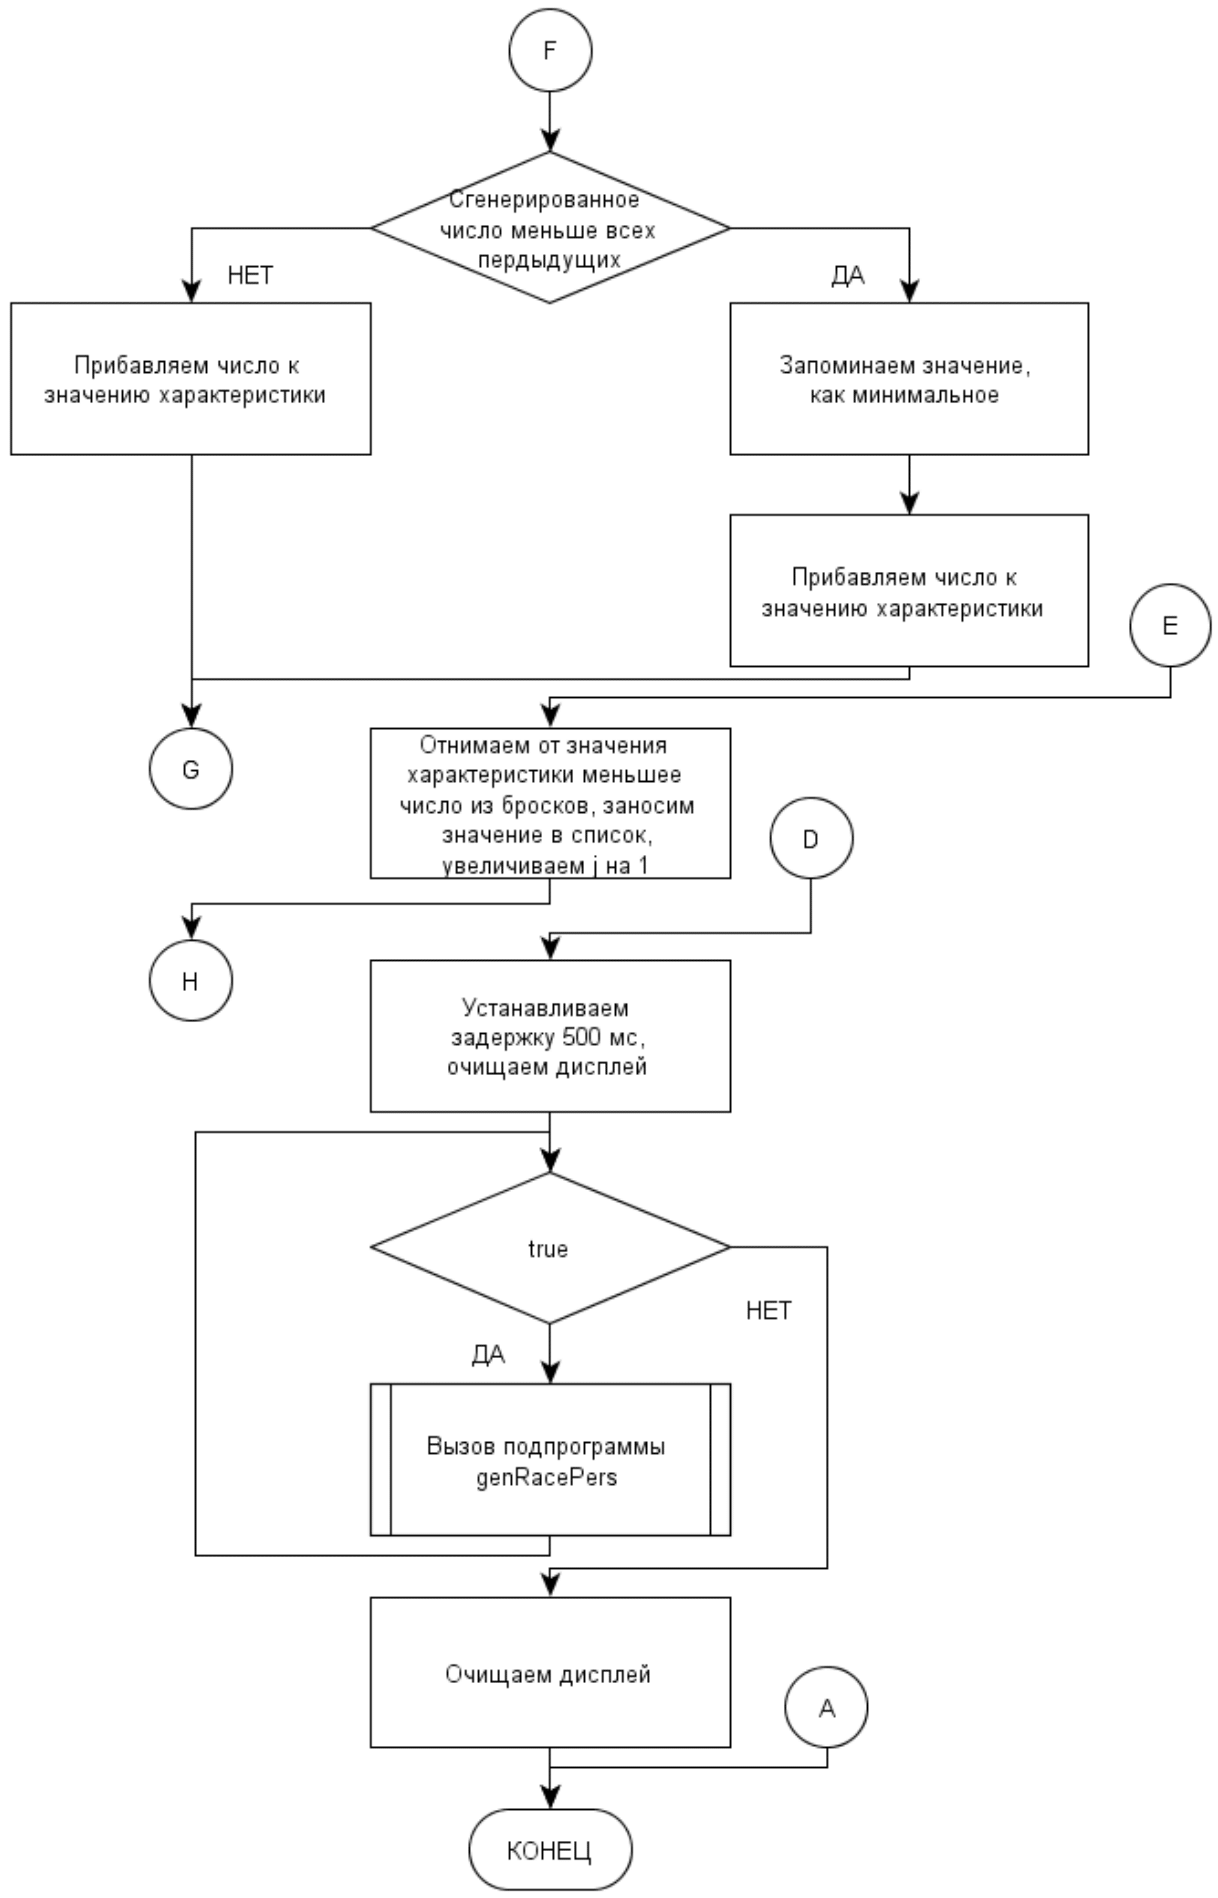
\includegraphics[scale=1]{mainText2.png}
    \caption{Блок-схема функции mainText}
    \label{fig:main2}
\end{figure}

\begin{figure}[H]
    \centering
    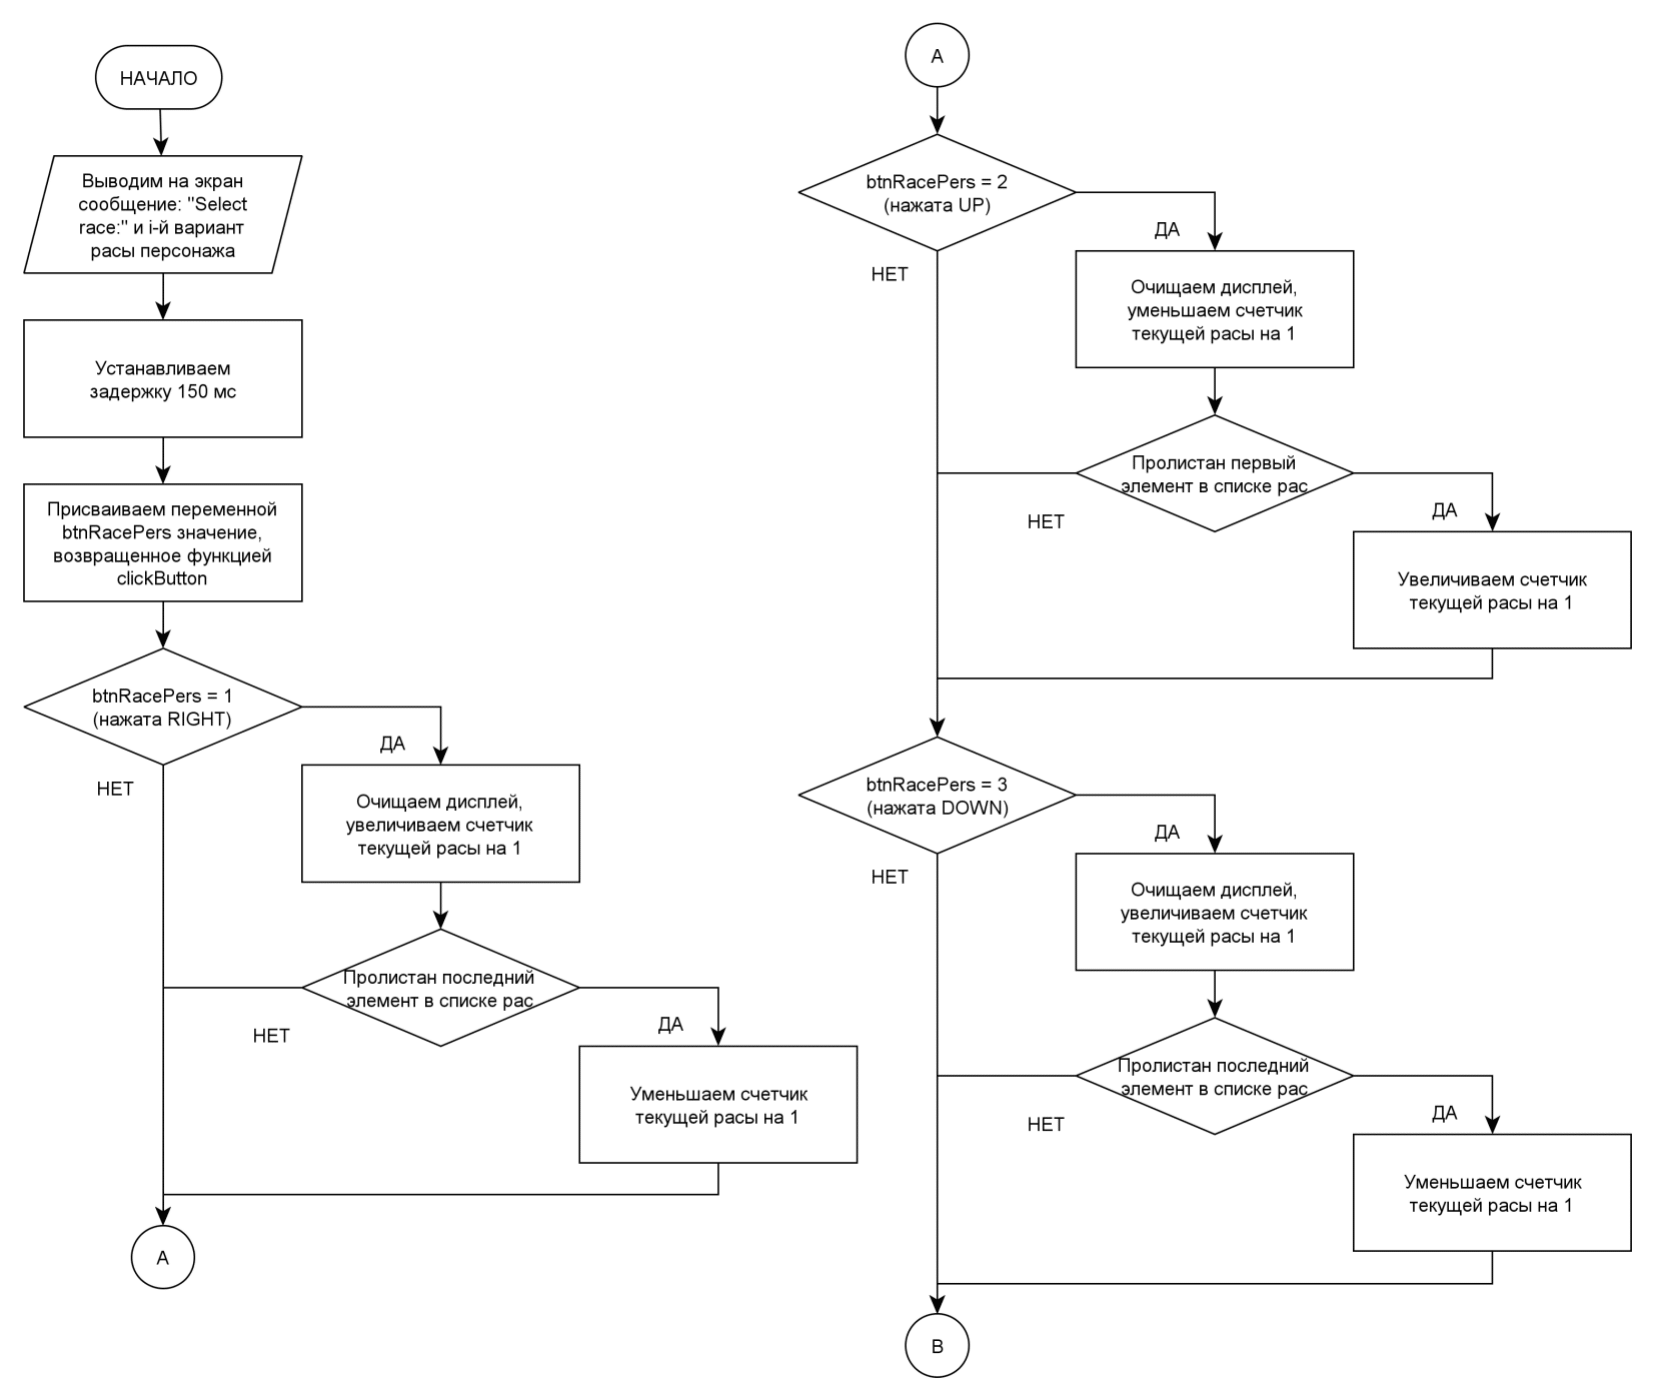
\includegraphics[scale=0.8]{genRacePers1.png}
    \caption{Блок-схема функции genRacePers}
    \label{fig:race1}
\end{figure}

\begin{figure}[H]
    \centering
    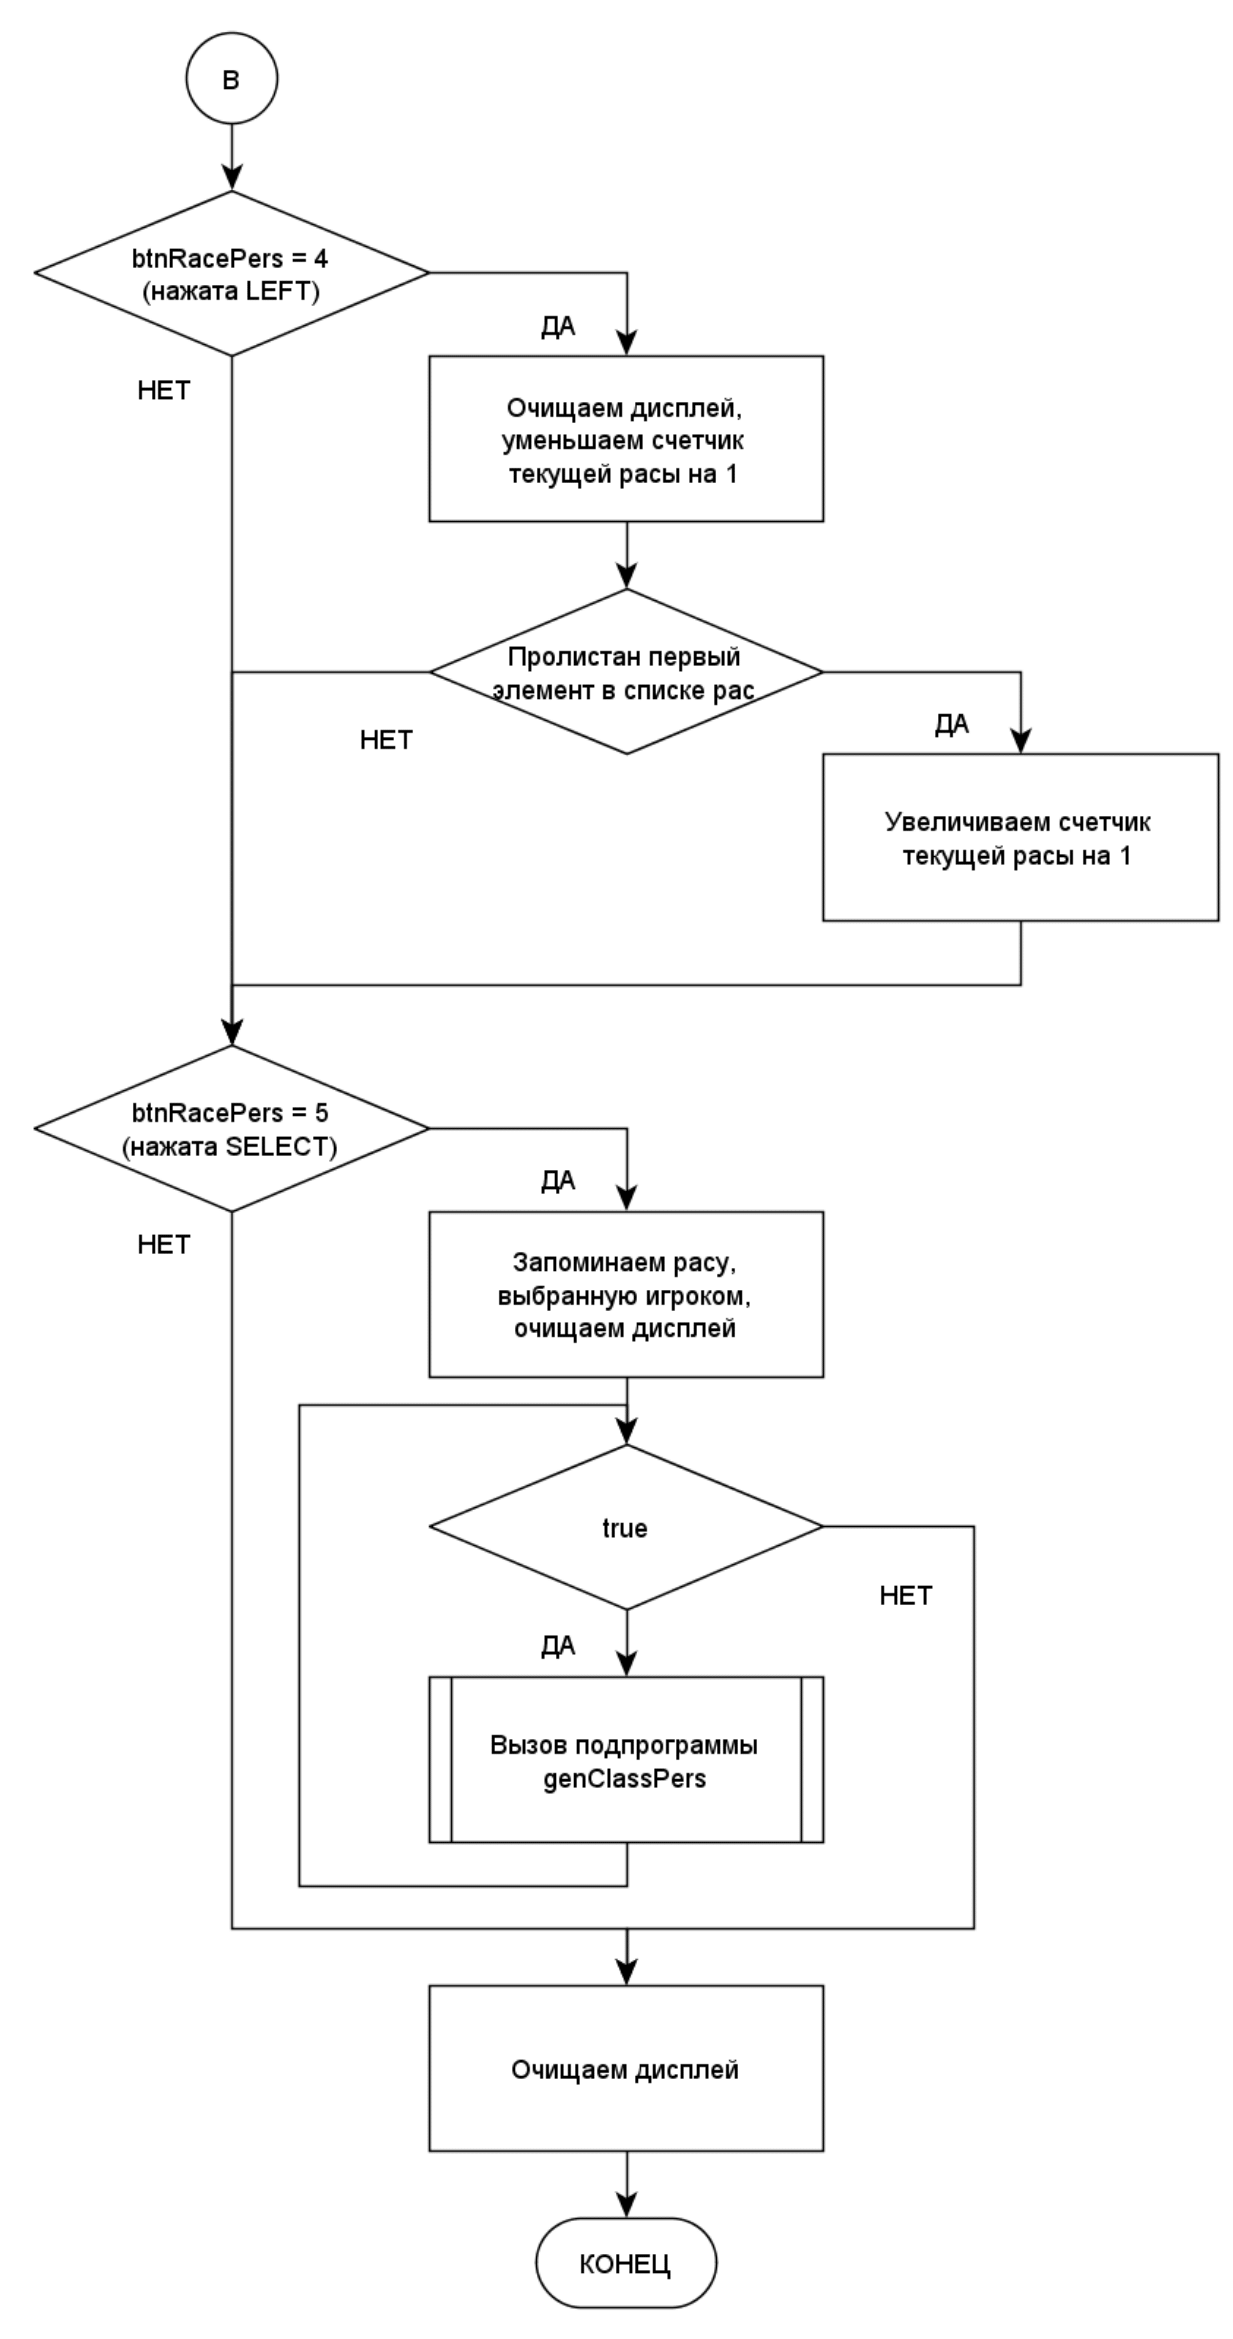
\includegraphics[scale=0.8]{genRacePers2.png}
    \caption{Блок-схема функции genRacePers}
    \label{fig:race2}
\end{figure}

\begin{figure}[H]
    \centering
    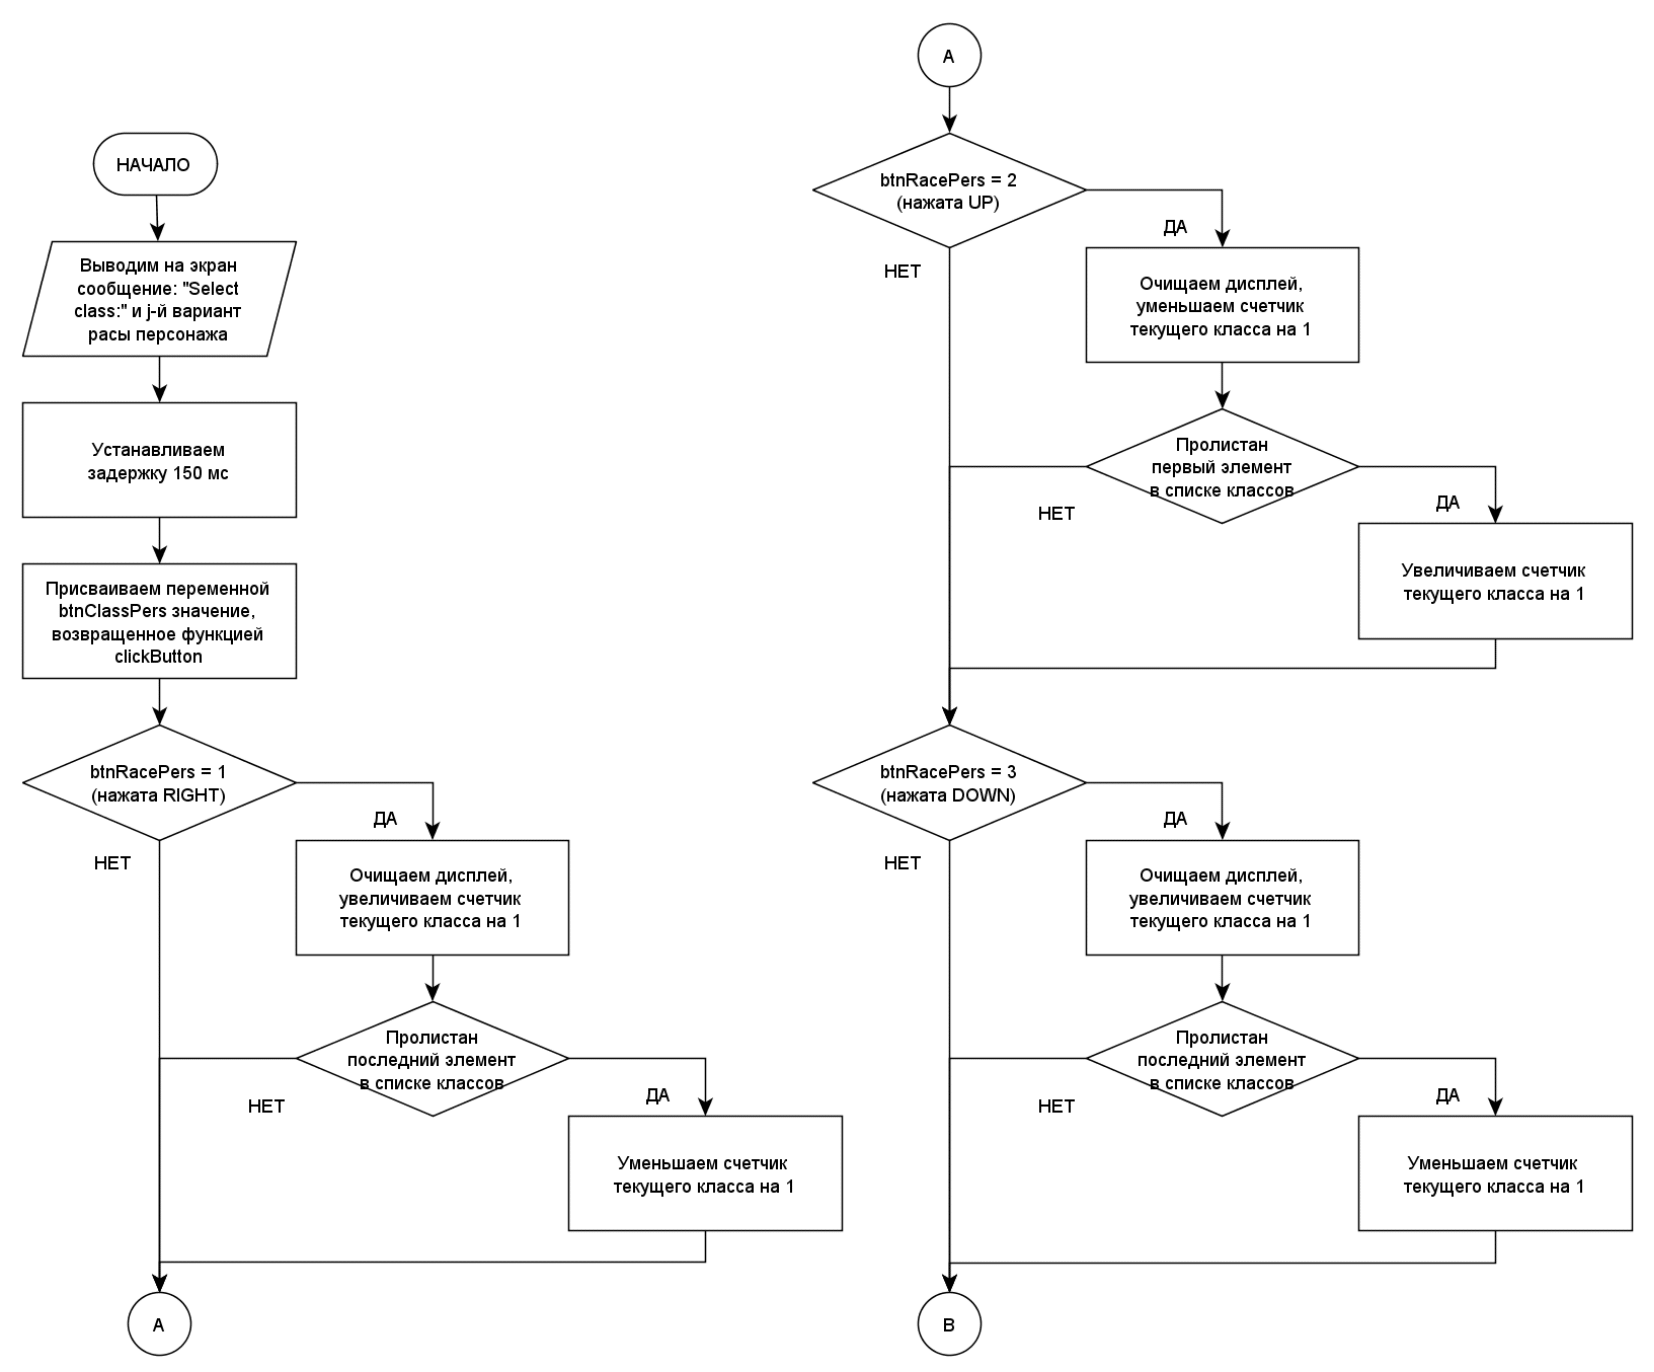
\includegraphics[scale=0.8]{genClassPers1.png}
    \caption{Блок-схема функции genClassPers}
    \label{fig:class1}
\end{figure}

\begin{figure}[H]
    \centering
    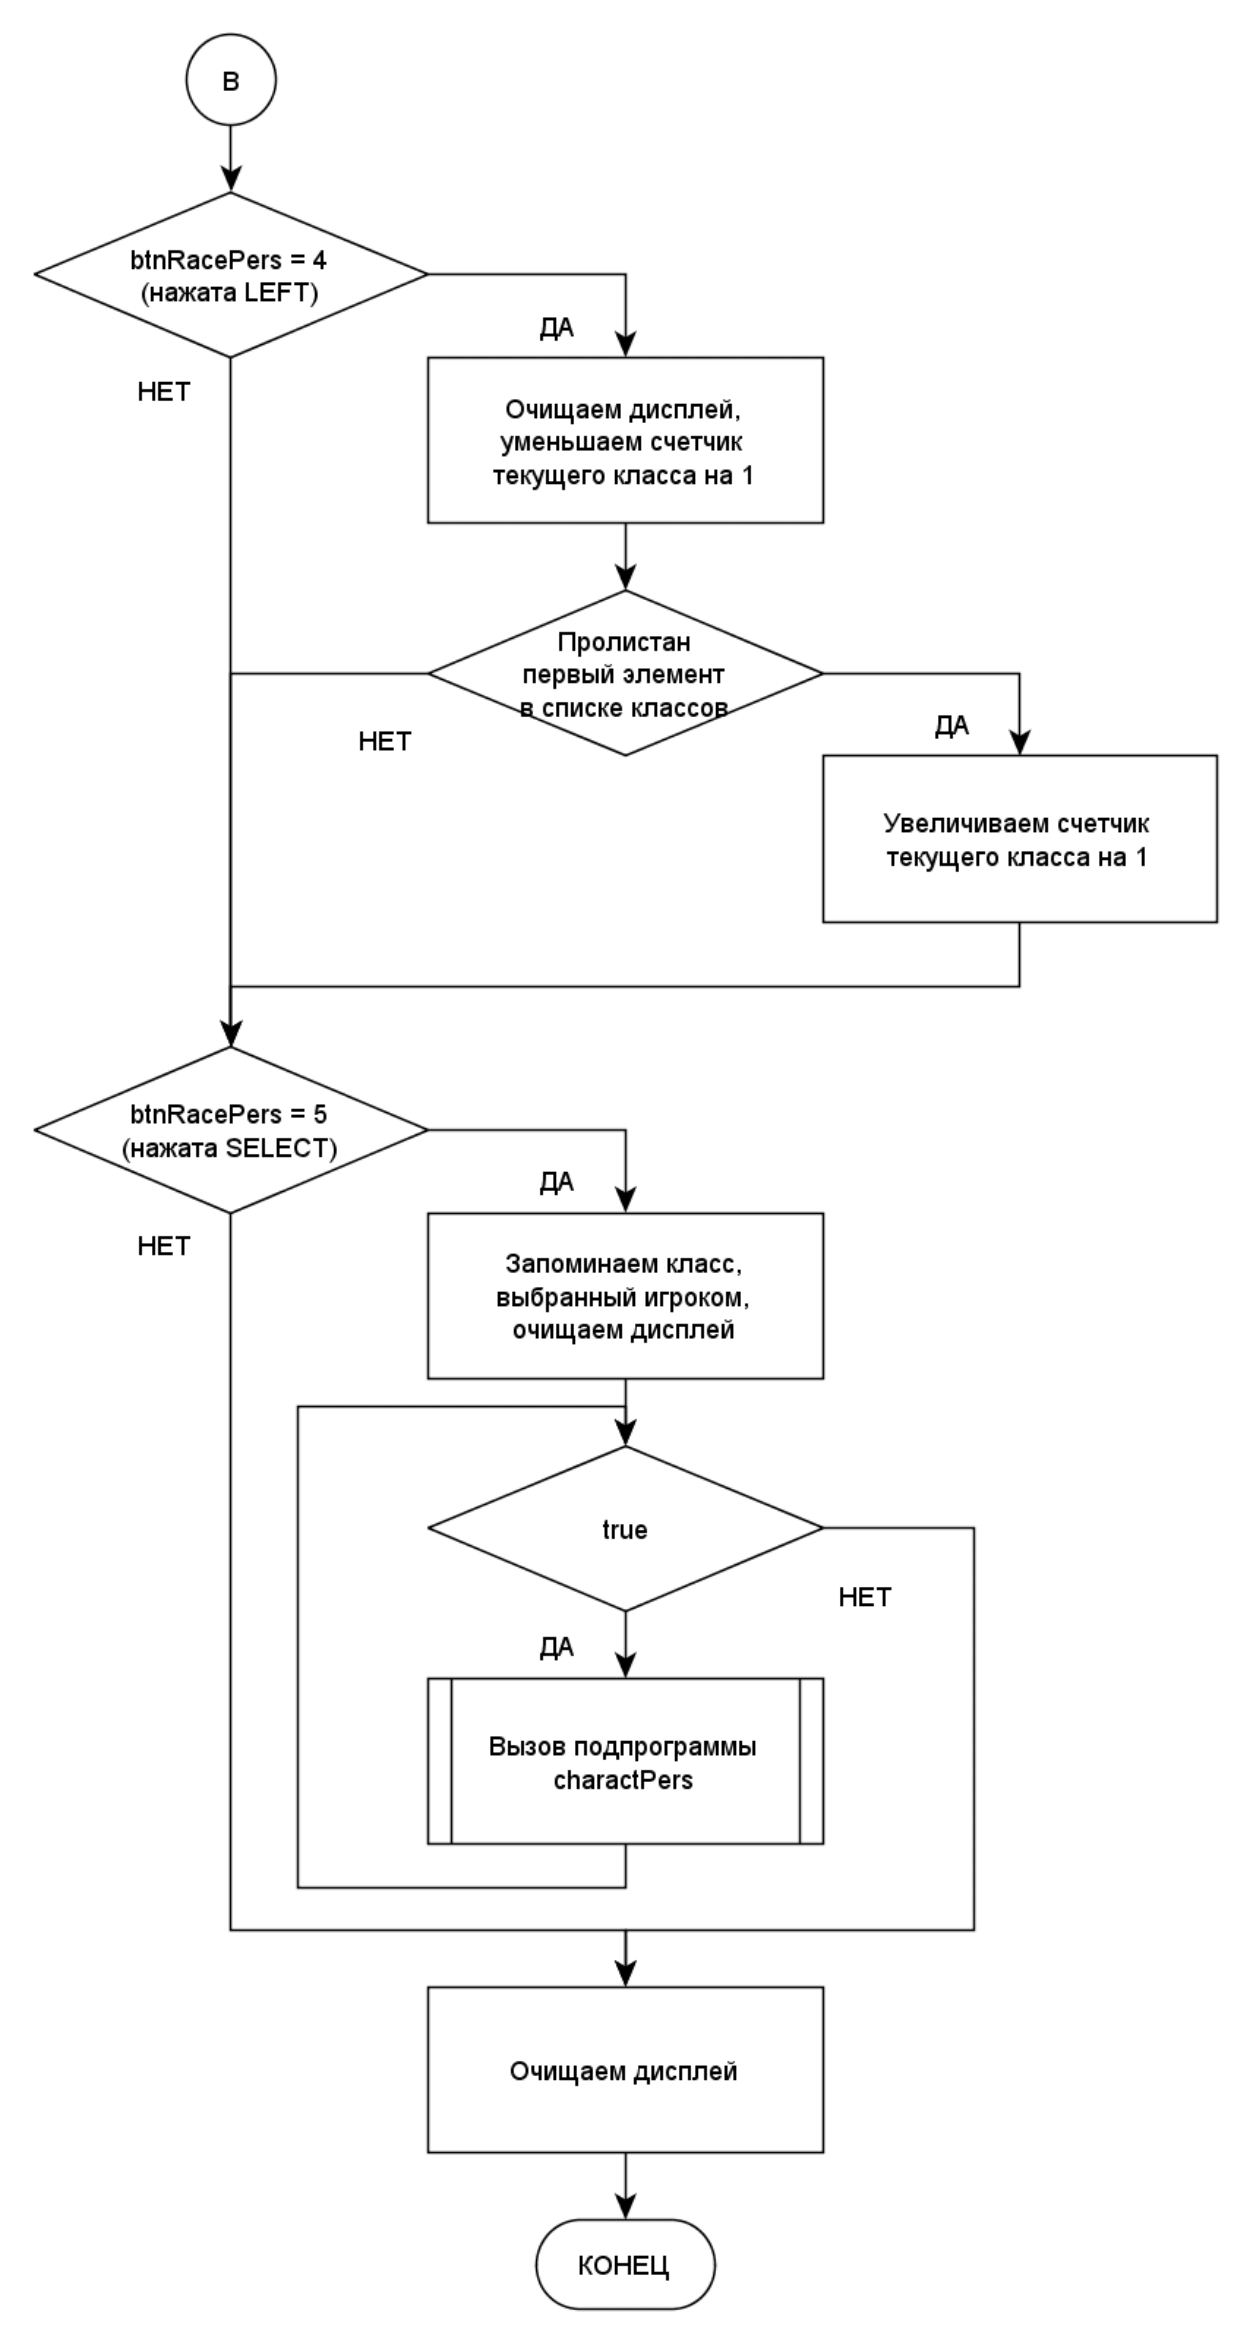
\includegraphics[scale=0.8]{genClassPers2.png}
    \caption{Блок-схема функции genClassPers}
    \label{fig:class2}
\end{figure}

\begin{figure}[H]
    \centering
    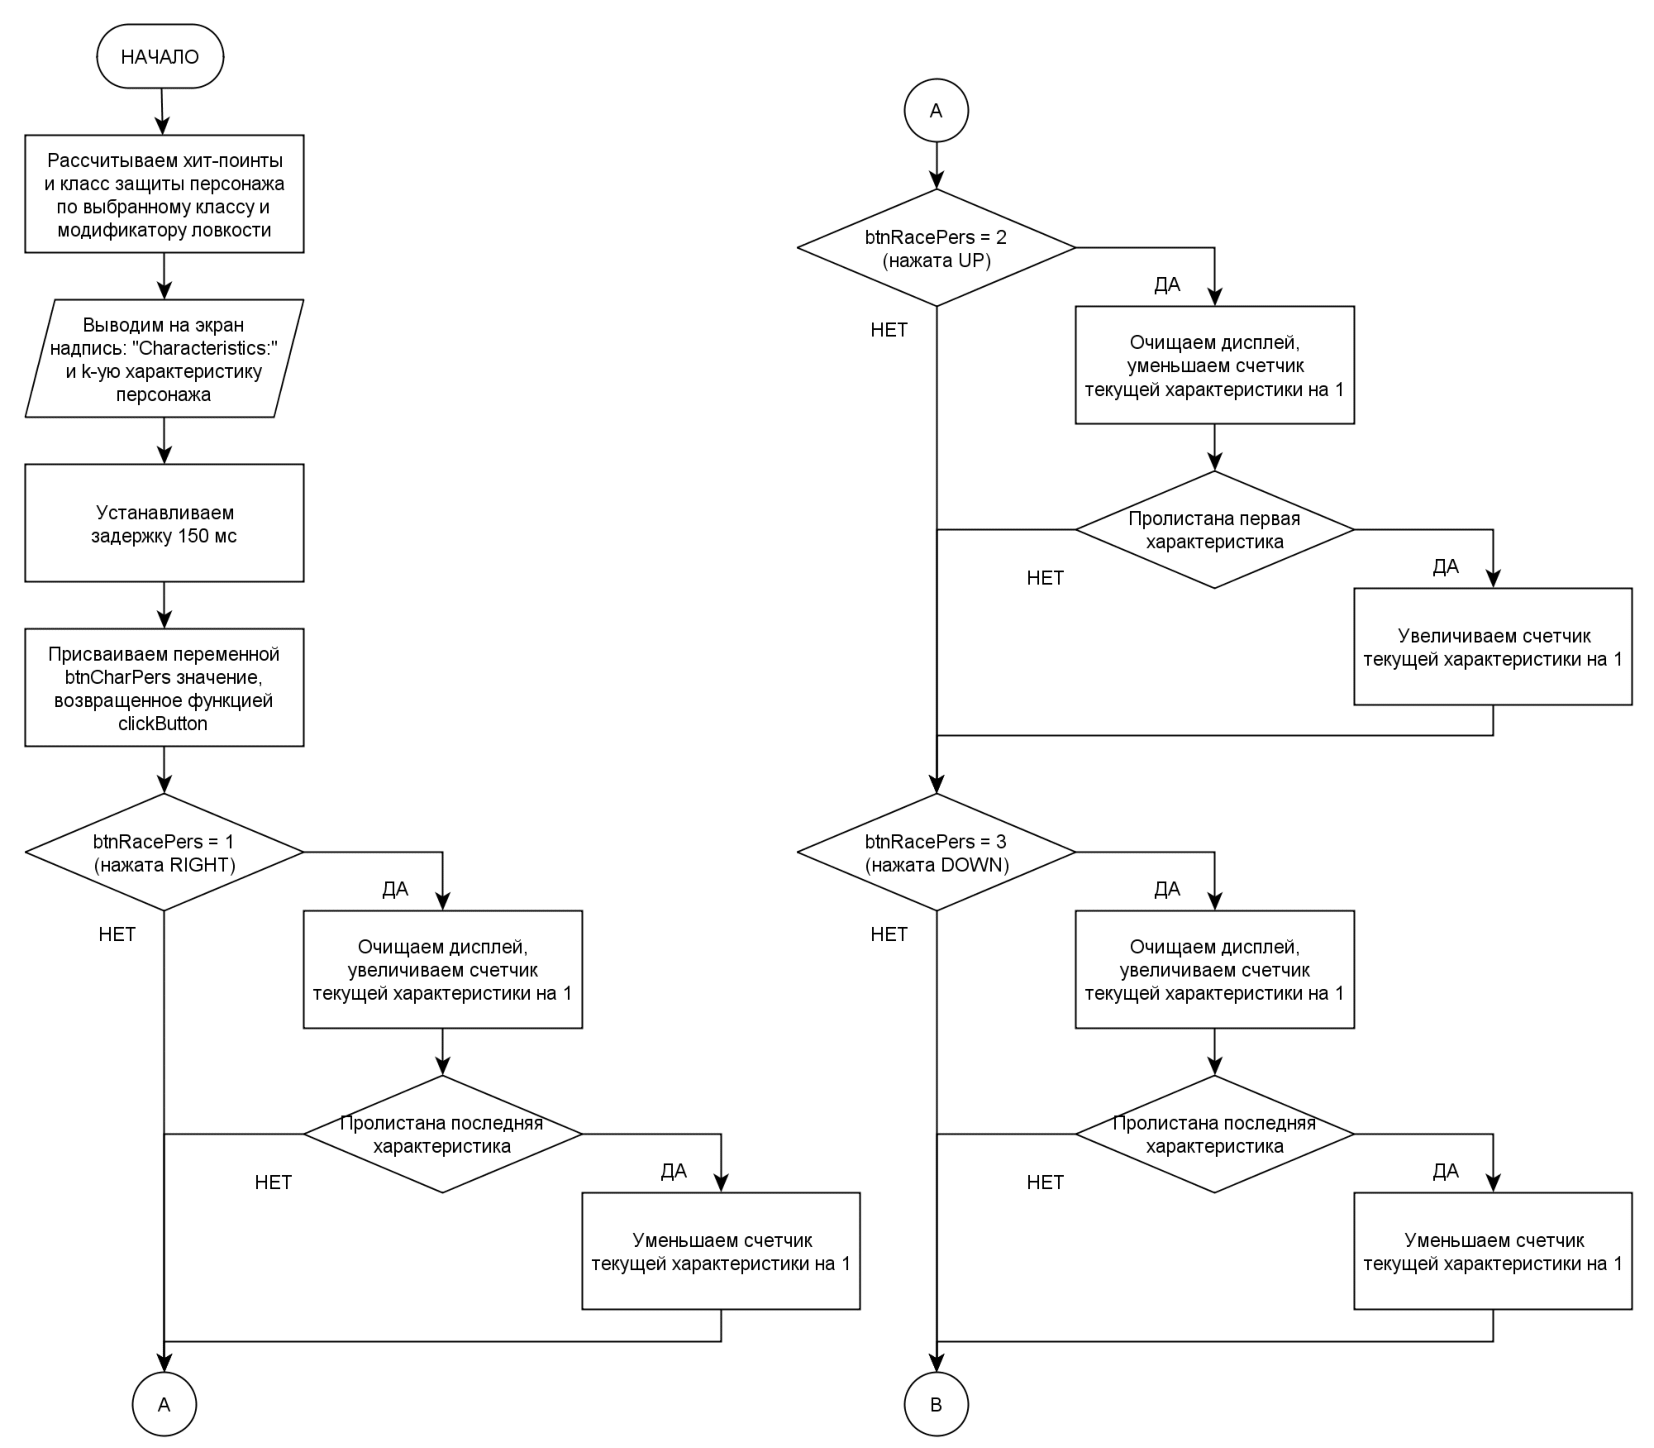
\includegraphics[scale=0.8]{charactPers1.png}
    \caption{Блок-схема функции charactPers}
    \label{fig:char1}
\end{figure}

\begin{figure}[H]
    \centering
    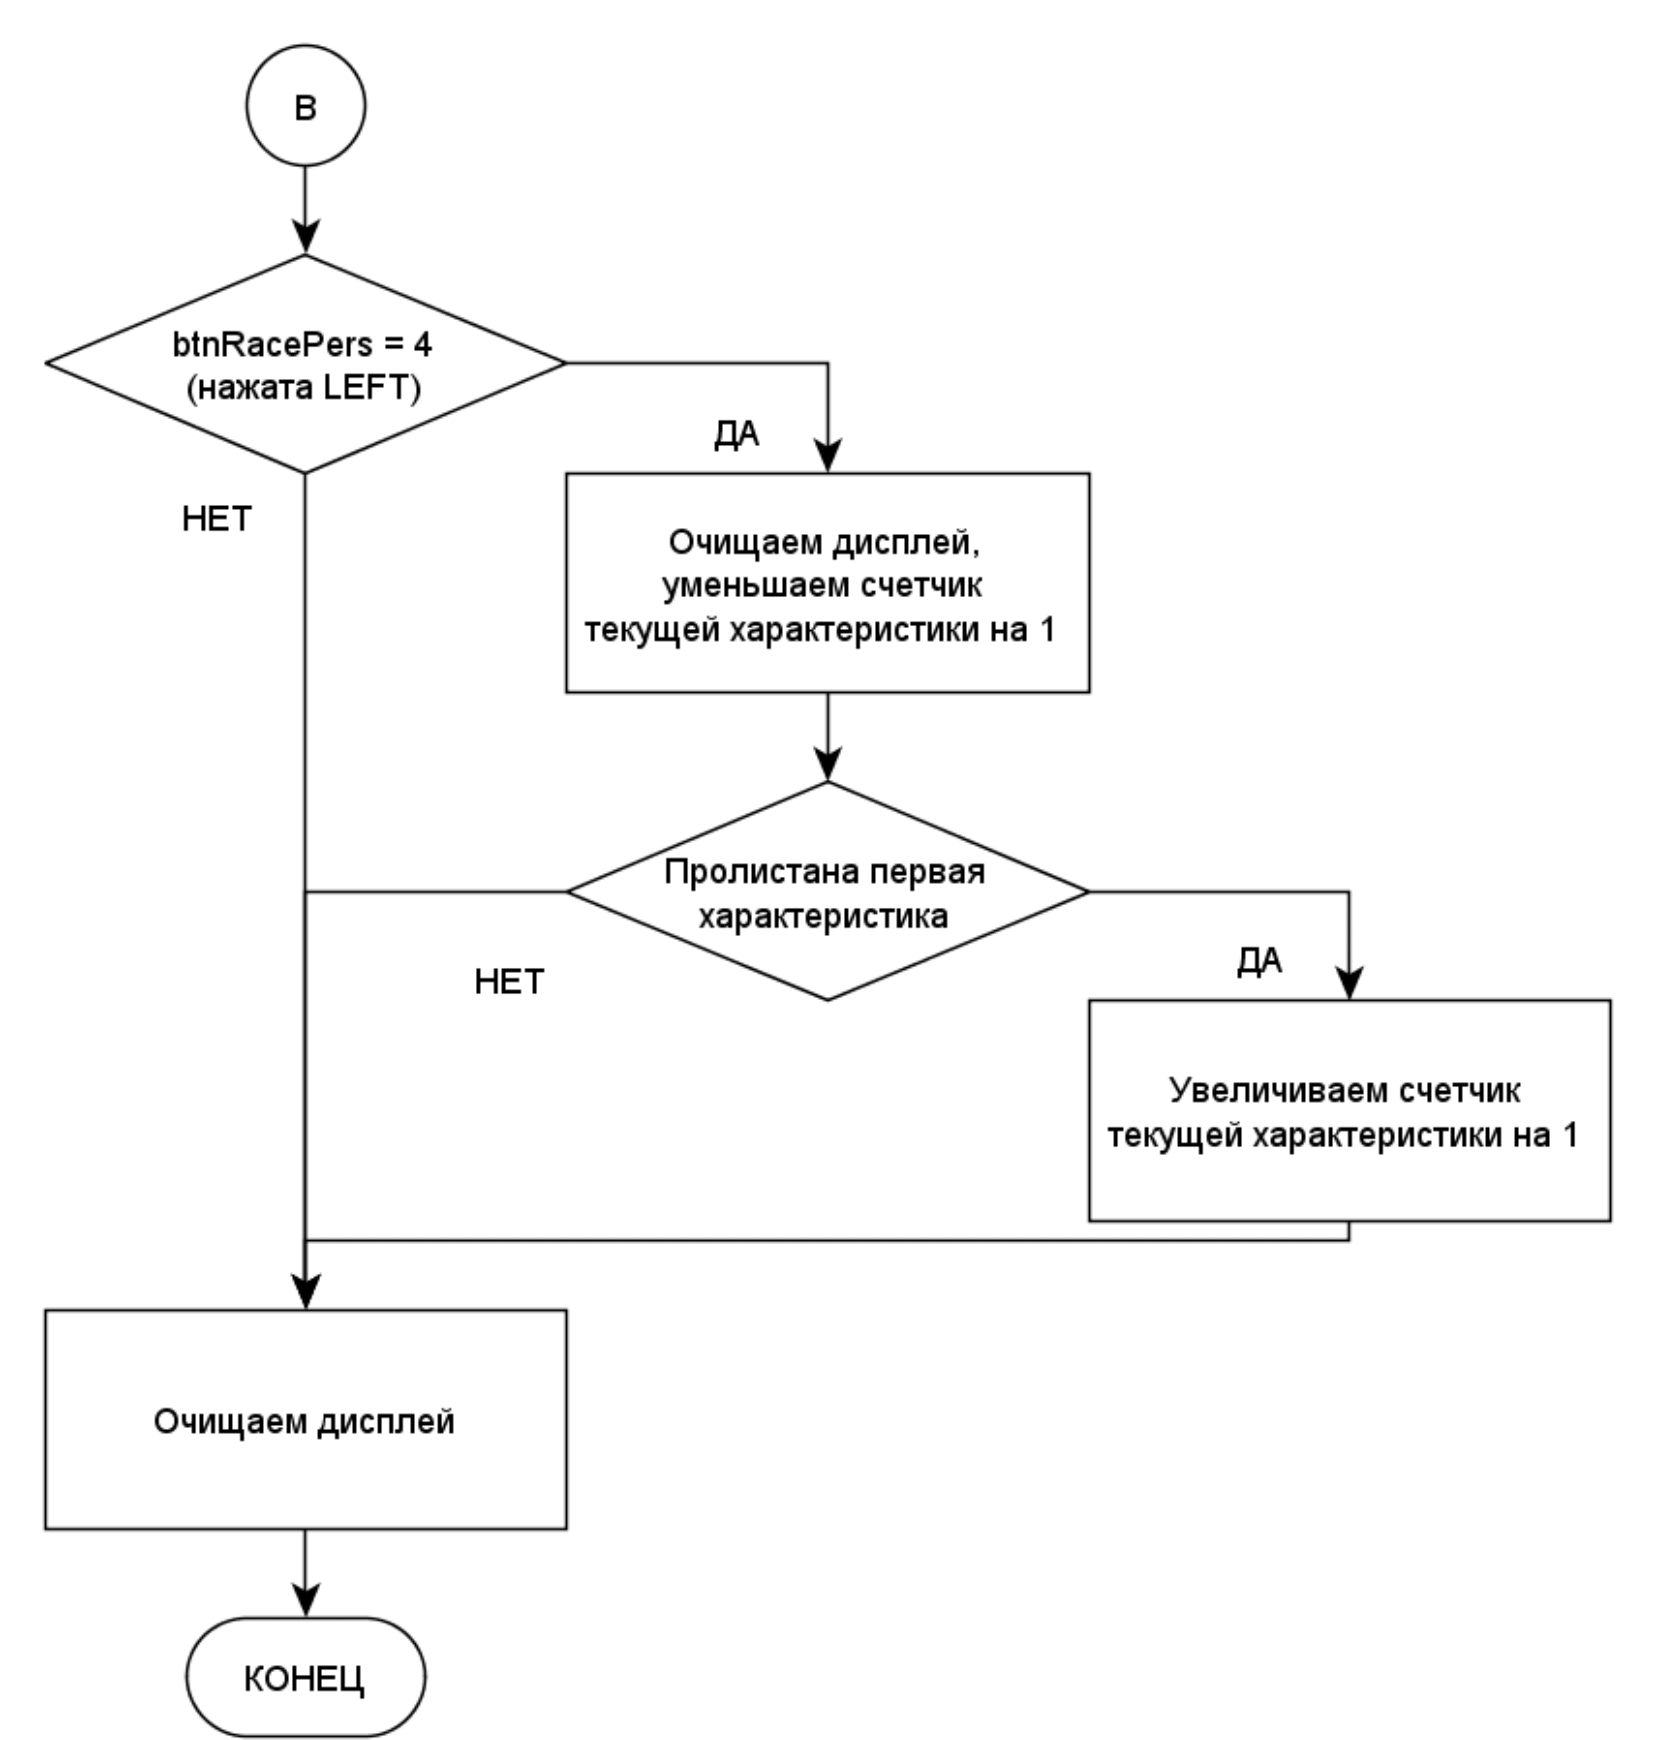
\includegraphics[scale=0.6]{charactPers2.png}
    \caption{Блок-схема функции charactPers}
    \label{fig:char2}
\end{figure}

\end{document}
